\documentclass{report}

\usepackage{../../../../../LaTeX/marzstyle}

\runningheads{Privacy and Data Security}{Exercise 02}

\setcounter{chapter}{2}


\begin{document}
	\pagestyle{fancy}
	\bibliographystyle{alphadin}
	\section{Privacy Policies}
	\startsection
		\subsection{Free Social-Network, Communication, or News App that drives revenue from advertisements (Instagram) \cite{InstagramPP}}
		\startsubsection
			Instagram is a social media platform, that is part of the Facebook group, in which a user can upload photos, follow other people or groups and chat with those as well. It gathers information about the user, i.e. information about the interests, actions and connections to select and personalize the advertisements, offers, and other sponsored content. Additionally location-based information, such as the current location, where the user lives, the places the user likes to visit, and the businesses and people in there area, are gathered to improve the advertisements. Because Instagram is part of the Facebook group it can combine information from both platforms to provide a more consistent experience.
		\closesection
		\subsection{Free Social-Network, Communication, or News App that does not rely on advertisements (Signal Messenger) \cite{SignalPP}}
		\startsubsection
			Signal itself does not gather much information about the user. The chat messages themselves are end-to-end encrypted such that Signal cannot access the content of messages or calls. Also information that were colected, like name, phone number are only shared with third parties in case of governmental or law enforcement request.
		\closesection
	\closesection
	
	\section{App-Specific Privacy Information}
	\startsection
		\subsection{20 Minuten App \cite{20MinutenAppStore}}
		\startsubsection
			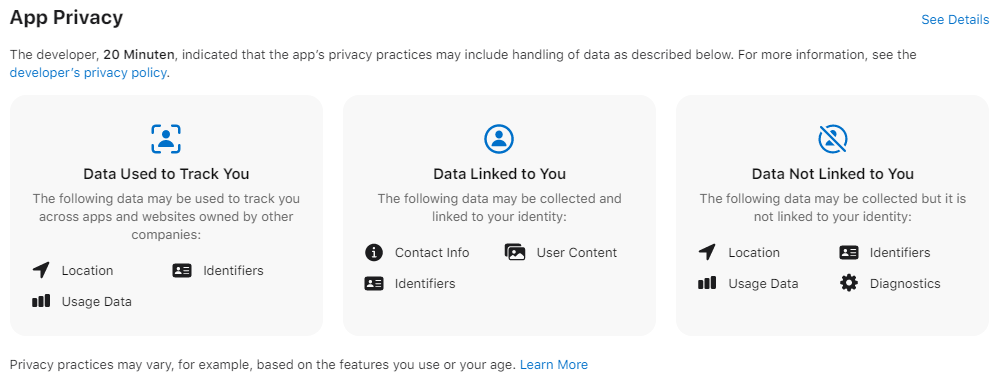
\includegraphics[scale=0.4]{20_Minuten_AppPrivacy.png}
		\closesection
		\subsection{Blick App \cite{BlickAppStore}}
		\startsubsection
			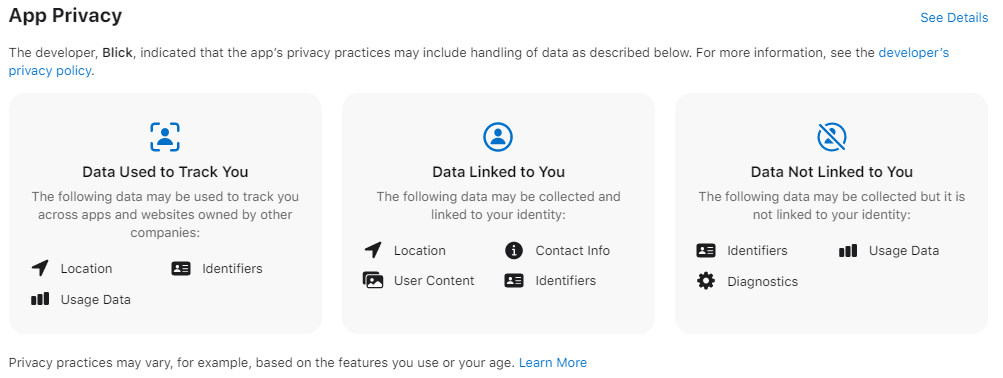
\includegraphics[scale=0.4]{Blick_AppPrivacy.png}
		\closesection
		\subsection{Frankfurter Allgemeine Zeitung App \cite{FAZAppStore}}
		\startsubsection
			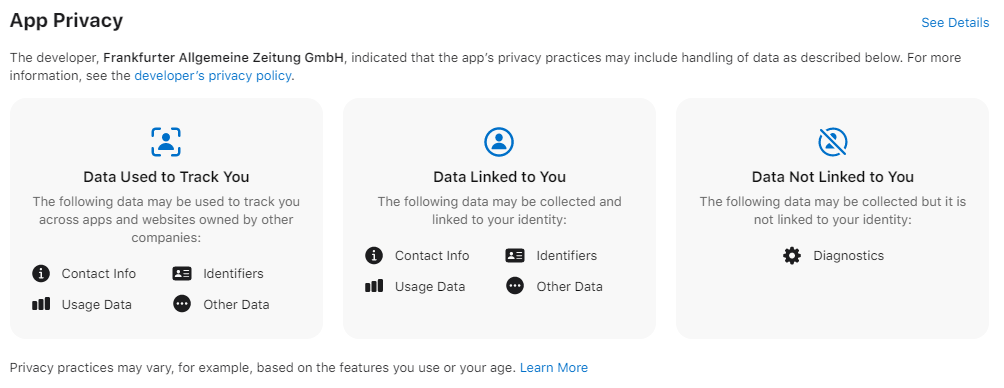
\includegraphics[scale=0.4]{FAZ_AppPrivacy.png}
		\closesection
		\subsection{Neue Zürcher Zeitung App \cite{NZZAppStore}}
		\startsubsection
			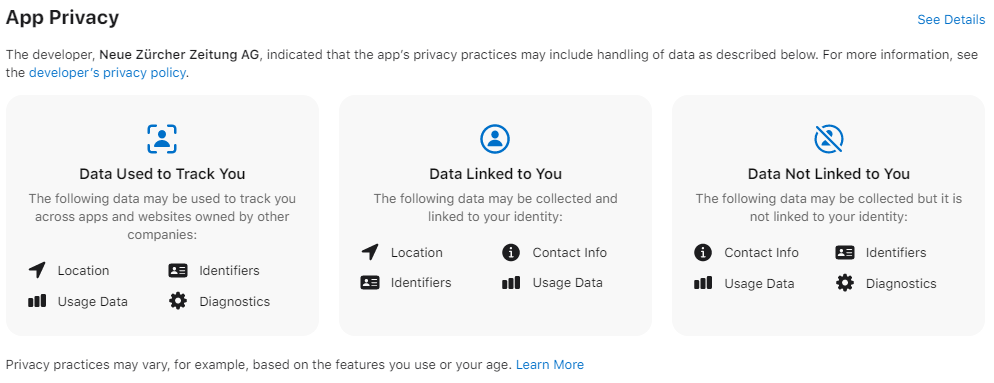
\includegraphics[scale=0.4]{NZZ_AppPrivacy.png}
		\closesection
		\subsection{Conclusion}
		\startsubsection
			All of the news paper applications are using location data in order to be able to track the user (Even the FAZ which is listing this under "Other Data"). Additionally all of the news apps collect identifiers and usage data. Only the location  data which is gather by 20 Minuten cannot be linked to the user, for all other apps this is not the case. For all apps in some regards they will collect data about contact info or user identifiers in order to be link to the user's identity. Also the 20 Minuten and Blick App do collect User Content. \\
			All of the news app are pretty similar in regards to which data are collected but some try to anonymize the data whereas the FAZ just take the data and directly link them to the user.
		\closesection
	\closesection
	
	\newpage
	{\let\clearpage\relax \bibliography{literature}}
\end{document}